% プロジェクト学習中間報告書書式テンプレート ver.1.0 (utf8)

% 両面印刷する場合は `openany' を削除する
\documentclass[openany,11pt,papersize]{jsbook}

% 報告書提出用スタイルファイル
%\usepackage[final]{funpro}%最終報告書
\usepackage[middle]{funpro}%中間報告書

% 画像ファイル (EPS, EPDF, PNG) を読み込むために
\usepackage[dvipdfmx]{graphicx,color}

% ファイル分割のためのパッケージ
\usepackage{subfiles}

% 参考文献管理
\usepackage[
  backend=biber,
  sorting=none,
  style=ieee
]{biblatex}
\addbibresource{ref.bib}

% ここから -->
\usepackage{calc,ifthen}
\newcounter{hoge}
\newcommand{\fake}[1]{\whiledo{\thehoge<70}{#1\stepcounter{hoge}}%
  \setcounter{hoge}{0}}
% <-- ここまで 削除してもよい

% 年度の指定
\thisYear{2017}

% プロジェクト名
\jProjectName{ビーコンIoTで函館のまちをハックする}

% [簡易版のプロジェクト名]{正式なプロジェクト名}
% 欧文のプロジェクト名が極端に長い(2行を超える)場合は、短い記述を
% 任意引数として渡す。
%\eProjectName[Making Delicious curry]{How to make delicious curry of Hakodate}
\eProjectName{Leverage the Beacon IoT in Hakodate Real Downtown for Our Smarter Life}


% <プロジェクト番号>-<グループ名>
\ProjectNumber{8-B}

% グループ名
\jGroupName{Youbeacomm}
\eGroupName{Youbeacomm}

% プロジェクトリーダ
\ProjectLeader{1015253}{橋場保鷹}{Hodaka~Hashiba}

% グループリーダ
\GroupLeader  {1015215}{藤原祐汰}{Yuta~Fujiwara}

% メンバー数
\SumOfMembers{5}
% グループメンバ
\GroupMember  {1}{1015074}{河田歩美}{Ayumi~Kawada}
\GroupMember  {2}{1015215}{藤原祐汰}{Yuta~Fujiwara}
\GroupMember  {3}{1015240}{荒田啓太郎}{Keitaro~Arata}
\GroupMember  {4}{1015250}{高橋大輔}{Daisuke~Takahashi}
\GroupMember  {5}{1015253}{橋場保鷹}{Hodaka~Hashiba}


% 指導教員
\jadvisor{松原克弥,藤野雄一,鈴木恵二,奥野拓}
% 複数人数いる場合はカンマ(,)で区切る。カンマの前後に空白は入れない。
\eadvisor{Katsuya~Matsubara,Yuichi~Fujino,Keiji~Suzuki,Taku~Okuno}

% 論文提出日
\jdate{2017年7月26日}
\edate{July~21, 2017}

\begin{document}
%
% 表紙
\maketitle

%前付け
\frontmatter

% 和文概要
\begin{jabstract}

% プロジェクト全体の日本語概要
\subfile{mid-report-common/common-jabstract}

グループBは、フィールドワークから外国人観光客への言語の対応が必要と考え、外国人観光客が日本人とスムーズに会話できるように手助けをするためのスマートフォン向けのアプリケーションを作成することを目的とした。この問題を解決するために指さし会話帳というものがある。しかし既存の指さし会話帳では、自分が欲しいフレーズをすぐ見つけられない、欲しいフレーズが掲載されていないなどの課題がある。ここから、ビーコンで利用者のコンテキストを読み取り、そこから欲しい情報をしスマートフォンにアプリケーションから送信するというサービスを提案した。アイディアコンテスト時の名前は「Contextual 指さし会話帳」であったが、「指さし会話帳」は既に商標登録されているため、このアプリケーションの名前を「Youbeacomm」(ユビーコム)と改名した。
しかしこの提案を7月14日に行われた中間報告会で発表したところ、たくさんの課題が見つかった。後期では課題をもとにグループで提案を改善しアプリケーションを作成をする。そのアプリケーションを実際に外国人観光客に使用してもらい、レビューをいただく予定である。そしてこれを繰り返すことで外国人観光客のコミュニケーションを支援する。

% 和文キーワード
\begin{jkeyword}
  ビーコン, 函館, 外国人観光客, 指さし会話帳, コンテキスト
\end{jkeyword}
\bunseki{藤原祐汰}

\end{jabstract}

%英語の概要
\begin{eabstract}

% プロジェクト全体の英語概要
\subfile{mid-report-common/common-eabstract}

 Group B thought the correspondence of the languages from fieldwork to a foreign tourist was necessary. We help you so that a foreign tourist can talk with a Japanese smoothly. We are make an application for smartphones. This problem to solve use ``Pointing conversation book''. But it is not find out use phrase. We suggested smartphone apprication. This apprication is read the context of the user in a beacon and transmitted to smartphone from an apprication. We proposaled this apprication on July 14. We find out a lot of problems. We improve this problem and application.
This apprication use foregin tourist. We have review for foreign tourist.
We called ``Contextual Youbisashikaiwatyou'' when aidea contest. But it was already commercial law registration. So, we changed name ``Youbeacomm''.
% 英文キーワード
\begin{ekeyword}
  Beacon, Hakodate, Foreign Tourists, Pointing Conversation Book, Context
\end{ekeyword}
\bunseki{藤原祐汰}

\end{eabstract}

\tableofcontents% 目次


\mainmatter% 本文のはじまり

% プロジェクト共通の項目
\subfile{mid-report-common/common-chapters}


% グループごとの項目
\chapter{サービスの提案にあたって}

\section{背景}

\subsection{函館に訪れる外国人観光客}
 函館市は、北海道の中にある市の一つで人口はおよそ26万人の都市である。函館市は夜景や歴
史的建造物、温泉といった多くの観光地を持っているため、日本人だけではなく多くの外国人観光
客が訪れる。平成28年度における観光入込客数は、上期(4月~9月)は約366万5千人
(前年同期に比べ約45万4千人増の114.1%)、下期(10月~3月)は約194万2千人(約20万6千人増の111.9%)、合計約560万7千人(約66万人増の113.3%)となった。さらに
外国人宿泊客数については、台湾や中国だけでなく、近年はタイ、マレーシアなどの東南アジアか
らの宿泊客が増加し、全体でも約40万5千人(約7千人増、前年比101.9%) と過去最高を
更新した\cite{b}。
以上のことから、現在函館には多くの外国人観光客が訪れていることがわかる。しかし、外国人が函館を観光する上でさまざまな問題を抱えている。
\bunseki{藤原祐汰}

\subsection{函館の地元民と外国人観光客の意思疎通の問題}\label{sec:mokuteki}
 毎年多くの外国人観光客が訪れる中での問題点は、地元民がどう他言語に対応するかという問題である。母国語で話をしてくる外国人観光客が、何を伝えたいのか理解するのが難しく、同じ言語で会話するレベルでの意思疎通を図ることは非常に困難である。ここで情報センター出版局で出版されている「旅の指さし会話帳」(以下、指さし会話帳)というものがある。指さし会話帳とは、旅行中で頻繁に使われるフレーズが、日本語と外国語に訳されており、指をさすだけでコミュニケーションがとれるという会話集のことである。
この本は現在70以上の言語に対応できるようにシリーズ化されている。しかし既存の「指さし会話帳」には扱いにくい点が2つある。
1つ目は、掲載されているフレーズ多いということである。そのために、自分の伝えたいフレーズがどこに掲載されているのかわからず、本の扱いに慣れるまでは見つけにくいという点である。
2つ目は、掲載されているフレーズしか使えない点である。つまり本のなかに利用者のほしいフレーズがない場合、的確なコミュニケーションをとることができなのである。
\bunseki{藤原祐汰}

\section{目的}
 本グループは~\ref{sec:mokuteki}~で取り上げた既存の「指さし会話帳」の課題をビーコンで改善し、指さし会話帳を改良・発展させたスマートフォン向けのアプリ「Youbeacomm」を作成する。本グループは「Youbeacomm」を作成することが目的である。
\bunseki{藤原祐汰}


\chapter{Youbeacommについて}

\section{Youbeacommの概要}
 Youbeacommは外国人旅行者と日本人をつなぐコミュニケーション促進サービスとして、お互いに共通の言語がない人々に対し、そのコミュニケーションをソフトウェアによって支援する。
\ref{sec:mokuteki}~で述べたように、同様の課題への解決策として、「旅の指さし会話帳」という、様々なフレーズや単語が2言語で併記されている書籍が市販されている。
外国人旅行者はこの書籍に印刷されたフレーズや単語を指さすだけで、気軽に現地の人とコミュニケーションを行うことができる。
旅行中の様々な場面で使われていることを想定しているため、コンテンツは非常に充実しており、日常で発生するであろう大半のケースに対応している。
しかしながら、掲載されている情報量が多いことのデメリットとして、旅行先での各場面ごとに適切な情報を絞り込むことが困難であることがあげられる。
また、紙媒体である以上、同一のコンテンツを重複して掲載することは難しく、利用者の想像と全く異なるジャンルのページに掲載されていることもある。
例として、写真を撮ってもらいたい場合に使うフレーズが観光に関連するすべてのページ掲載されていれば、ページめくりは発生しないが、
実際には持ち運びやすい判型にするという紙面の都合上、「あいさつ」というジャンルに分類されている。

本提案手法では利用者の現在地や移動経路、時間帯、天候など、コミュニケーションで支援が必要となる状況と、
あらかじめ収集した場所の属性(商業施設、駅、市役所など)やその周辺の状況などを総合して、「コンテキスト」と呼ぶ。
それらをもとに利用者の置かれている環境を把握し、フレーズや単語の絞り込みや優先度付けを行うことで、利用者がその時点で正に求めている候補を提案することを目指す。
例として、利用者が空港の搭乗口から到着ロビーへ移動 (それぞれの場所に設置したビーコンを順に検知) したとする。
その場合、「空港に到着した後、ターミナル外に移動しようとしている」ものとして、路線バスやタクシーなどの移動手段についてのフレーズが求められるであろうと推定できるため、
交通に関係するフレーズに絞り込み、空港からの移動手段を優先的に表示する。
\begin{figure}[htbp]
 \begin{center}
  \makebox[\textwidth]{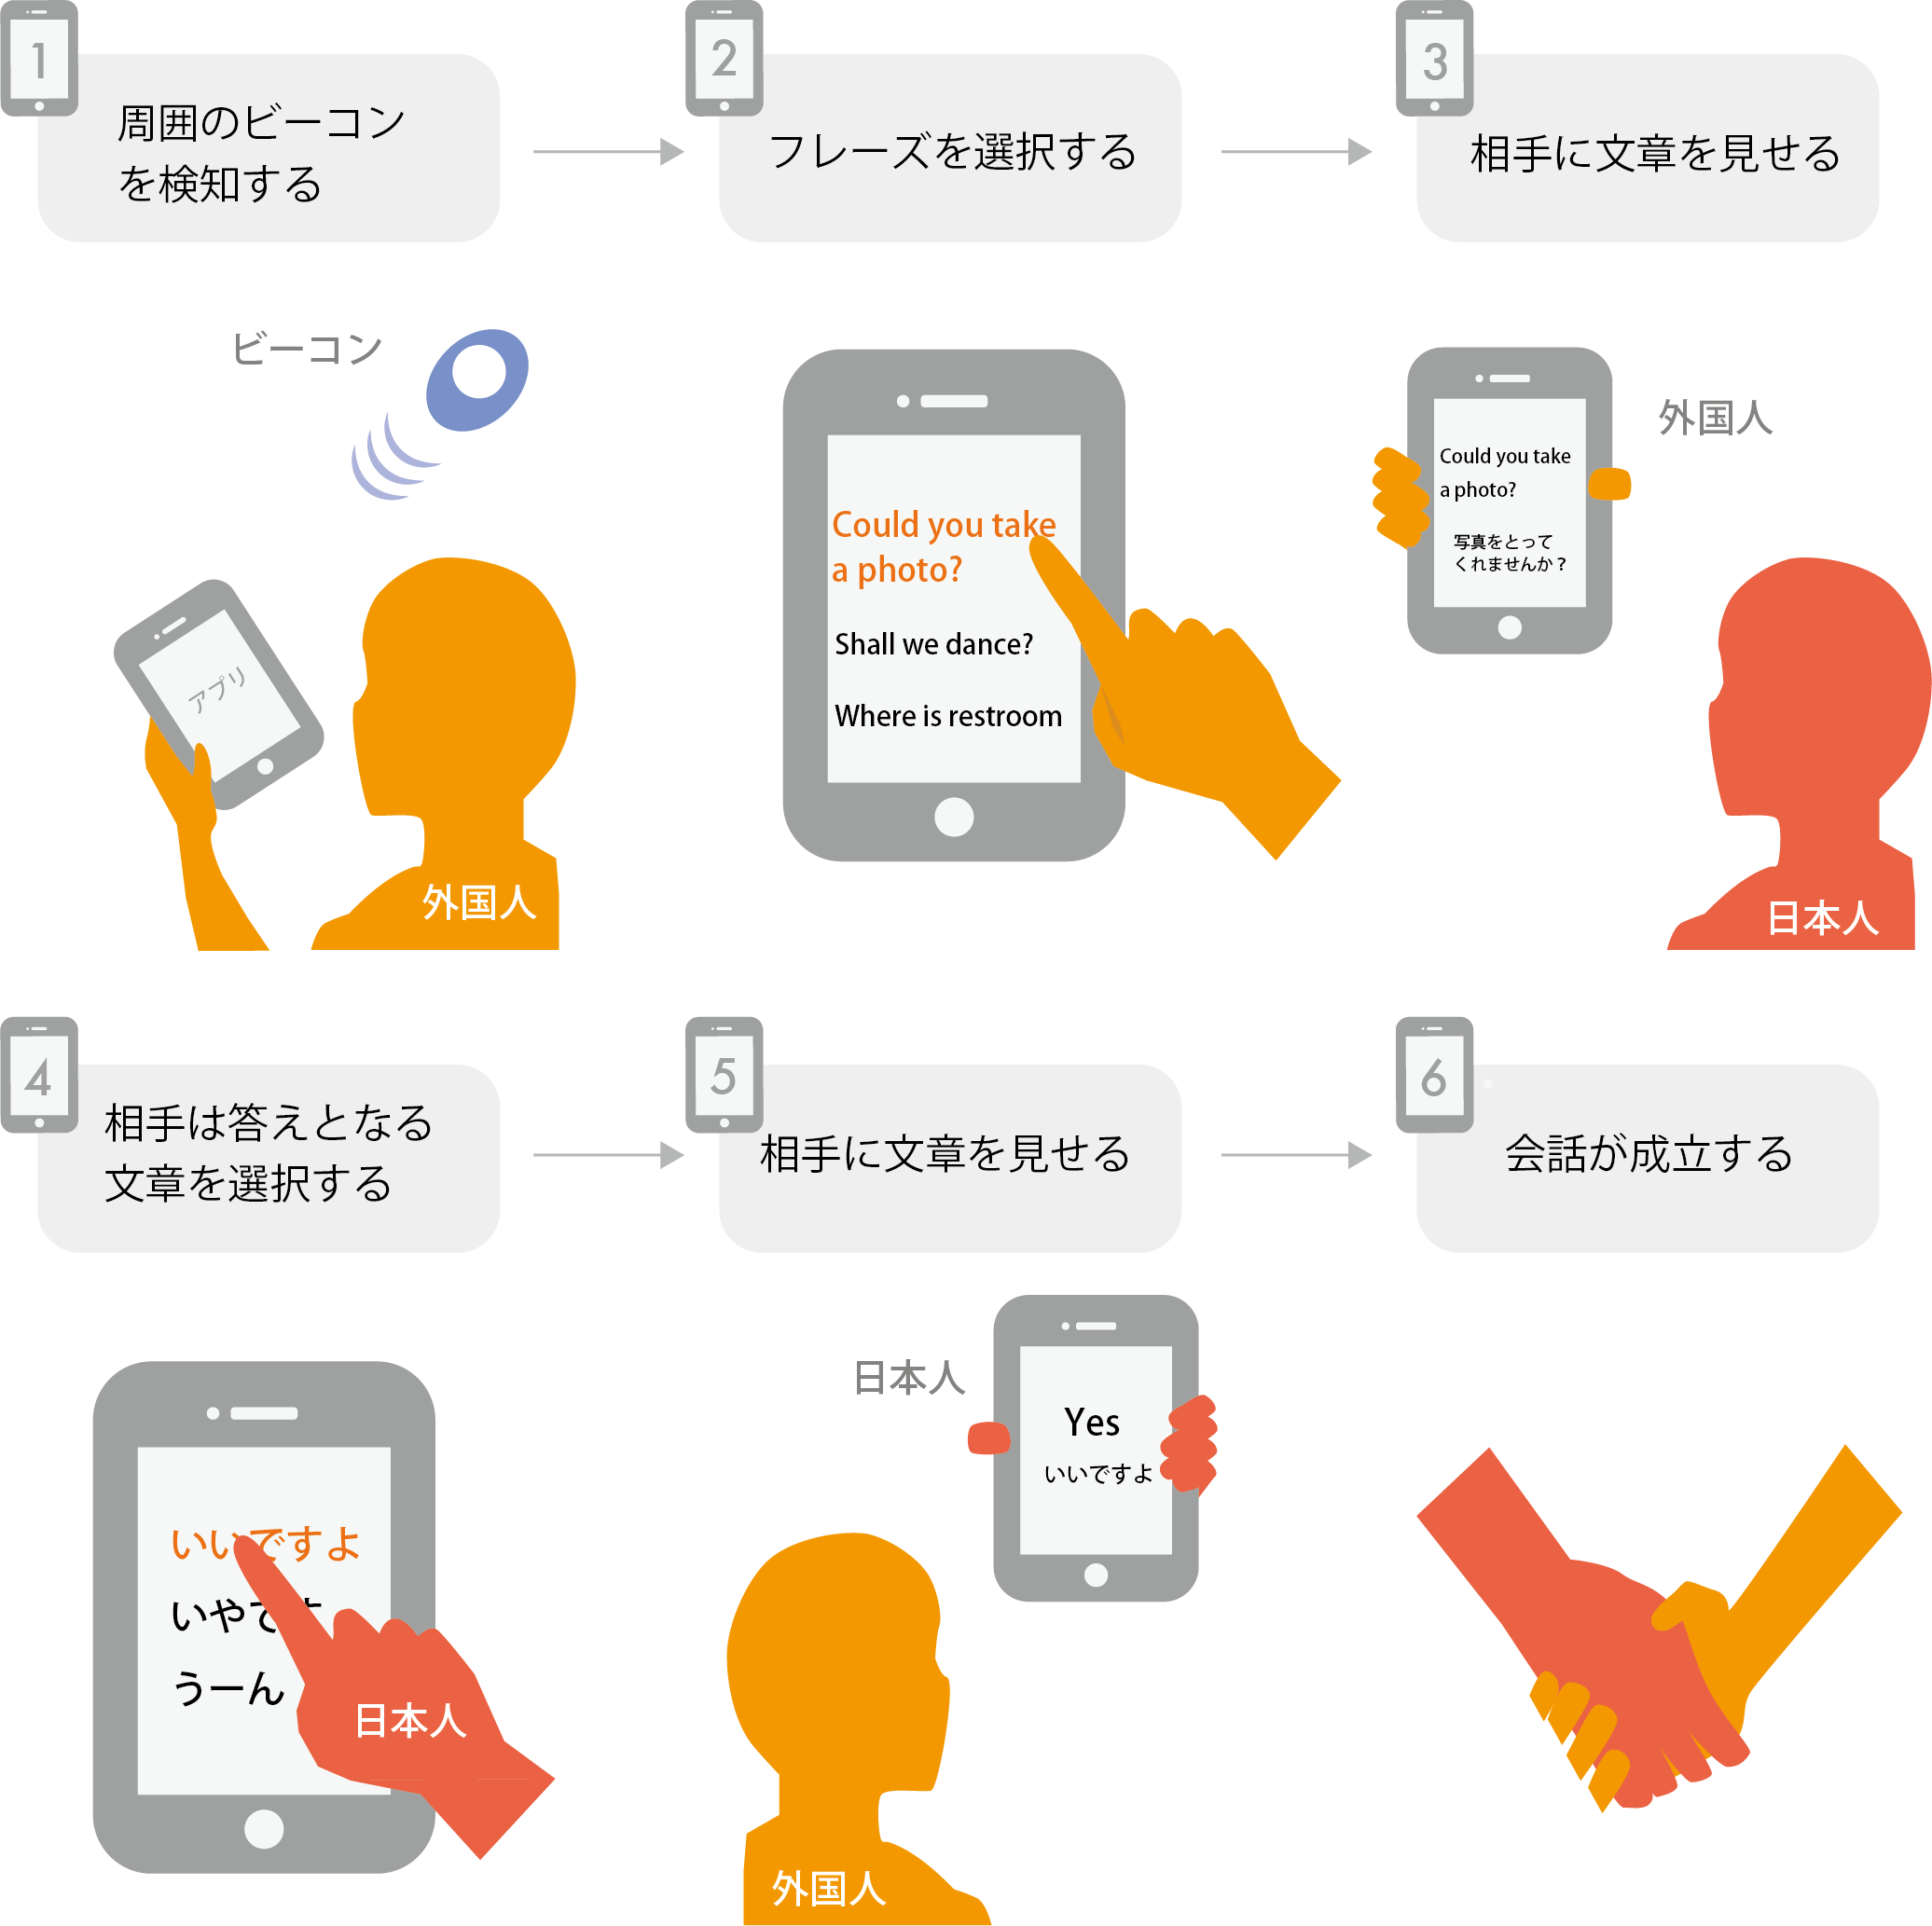
\includegraphics[width=0.75\paperwidth]{img/use_flow.png}}
 \end{center}
 \caption{提案するサービス}
 \label{fig:use_flow}
\end{figure}
\bunseki{高橋大輔}

\section{Youbeacommの具体的なシステムの説明}\label{sec:yonnoni}
 本システムへのアクセスは外国人旅行者向けのスマートフォンのアプリとして提供する。米Net Applications社のマーケットシェア調査\cite{c}によると、
世界の携帯端末の97.12%以上はAndroid (64.20%) かiOS (32.92%) を実行していることから、これら2つのOSを開発ターゲットとする。

アプリはGPS、(設置するビーコンを含む) BLE、Wi-Fiなどの情報をバックグラウンドで定期的に取得し、
利用者の起動操作によって、フォアグラウンドとなった時点で、それらの情報をサーバに送信する。
サーバはそれらをもとに位置情報や利用者周辺の環境を推定し、コンテキストを認識する。データベースに登録されているフレーズのうち、そのコンテキストにマッチするものを抜き出し、
コンテキストとフレーズの関係から優先度を計算して並び替えたリストを、アプリに対して応答することで、利用者に対してフレーズの提案が行われる。
利用者は、適切なフレーズを選択し、画面上に2か国語で表示された状態で、スマートフォンをコミュニケーションの相手 (日本語話者を想定) に渡して提示する。
サーバは選択された発話フレーズをコンテキストの1つとして考慮した上で、同様にデータベースからフレーズを提案する。コミュニケーションの相手も、
適切な回答フレーズを選択し、スマートフォンを利用者に返して提示することで、会話が成立する。

提案の中に適切なフレーズがない場合には、機械翻訳や観光案内所、電話による通訳サービスなどの案内を行うようにすることで、
利用者に対して常に複数の選択肢を提供しつつ、データの充実を主な目的として、これらのサービスとの様々な連係も行う。

また、適切なフレーズの提案がなかったこと自体については、提案されたフレーズに対して、利用者がフィードバックや追加の提案を行えるようにすることで、
フレーズの充実、並びに提案精度の向上を図る。

数百を超えるビーコンを効率的に管理するため、ビーコンなどの情報から位置情報等を推定するシステムには、簡易的な遠隔監視システムとしての役割を持たせる。
ビーコンが各利用者のスマートフォンに検知された事実や、ビーコンから一定の割合で通知される電池残量などの情報を、アプリを介して収集し、
検知された頻度や電池残量の推移などの得られた情報を用いることで、状態異常などを早期に把握し、効率的なメンテナンス計画の立案等につなげる。
\begin{figure}[htbp]
 \begin{center}
  \makebox[\textwidth]{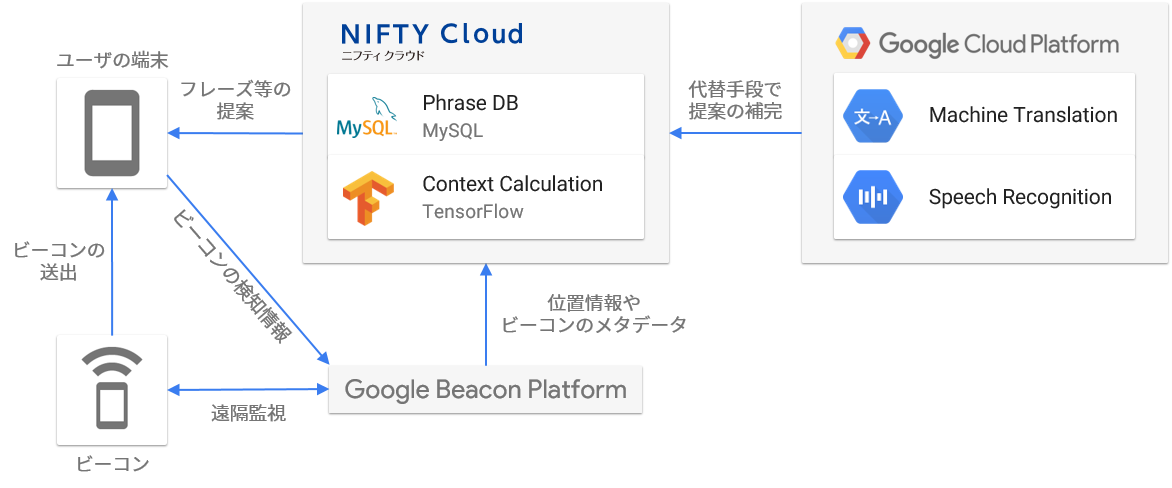
\includegraphics[width=0.75\paperwidth]{img/system_structure.png}}
 \end{center}
 \caption{システム構成図}
 \label{fig:system_structure}
\end{figure}
\bunseki{高橋大輔}

\section{現時点でのプロトタイプ}\label{sec:sannosan}
 中間報告会での説明のツールを兼ね、主要な機能の画面遷移を再現した14画面で構成される静的なプロトタイプの制作を行った。
このプロトタイプでは、アプリのインストールに誘導するプロモーションや実際のインストールなど、アプリの起動に至るまでのプロセスや、観光案内所などへの誘導のプロセスなどが
未再現ではあるものの、プロトタイピングツールを用いて制作する過程で、メンバー間でのアプリの機能に対する細部の認識を共有することができた。
今後、このプロトタイプをベースとして、動的にフレーズを提案する機能などを盛り込んだプロトタイプを制作したのち、その他の機能を順次実装していく。
その過程で、実際の外国人旅行者に使用・評価してもらい、利用者の需要を理解し、プロトタイプを制作するというプロセスを繰り返すことで、
利用者にとってより良いUXを提供できるシステムに近づけていく。
\begin{figure}[htbp]
 \begin{center}
  \makebox[\textwidth]{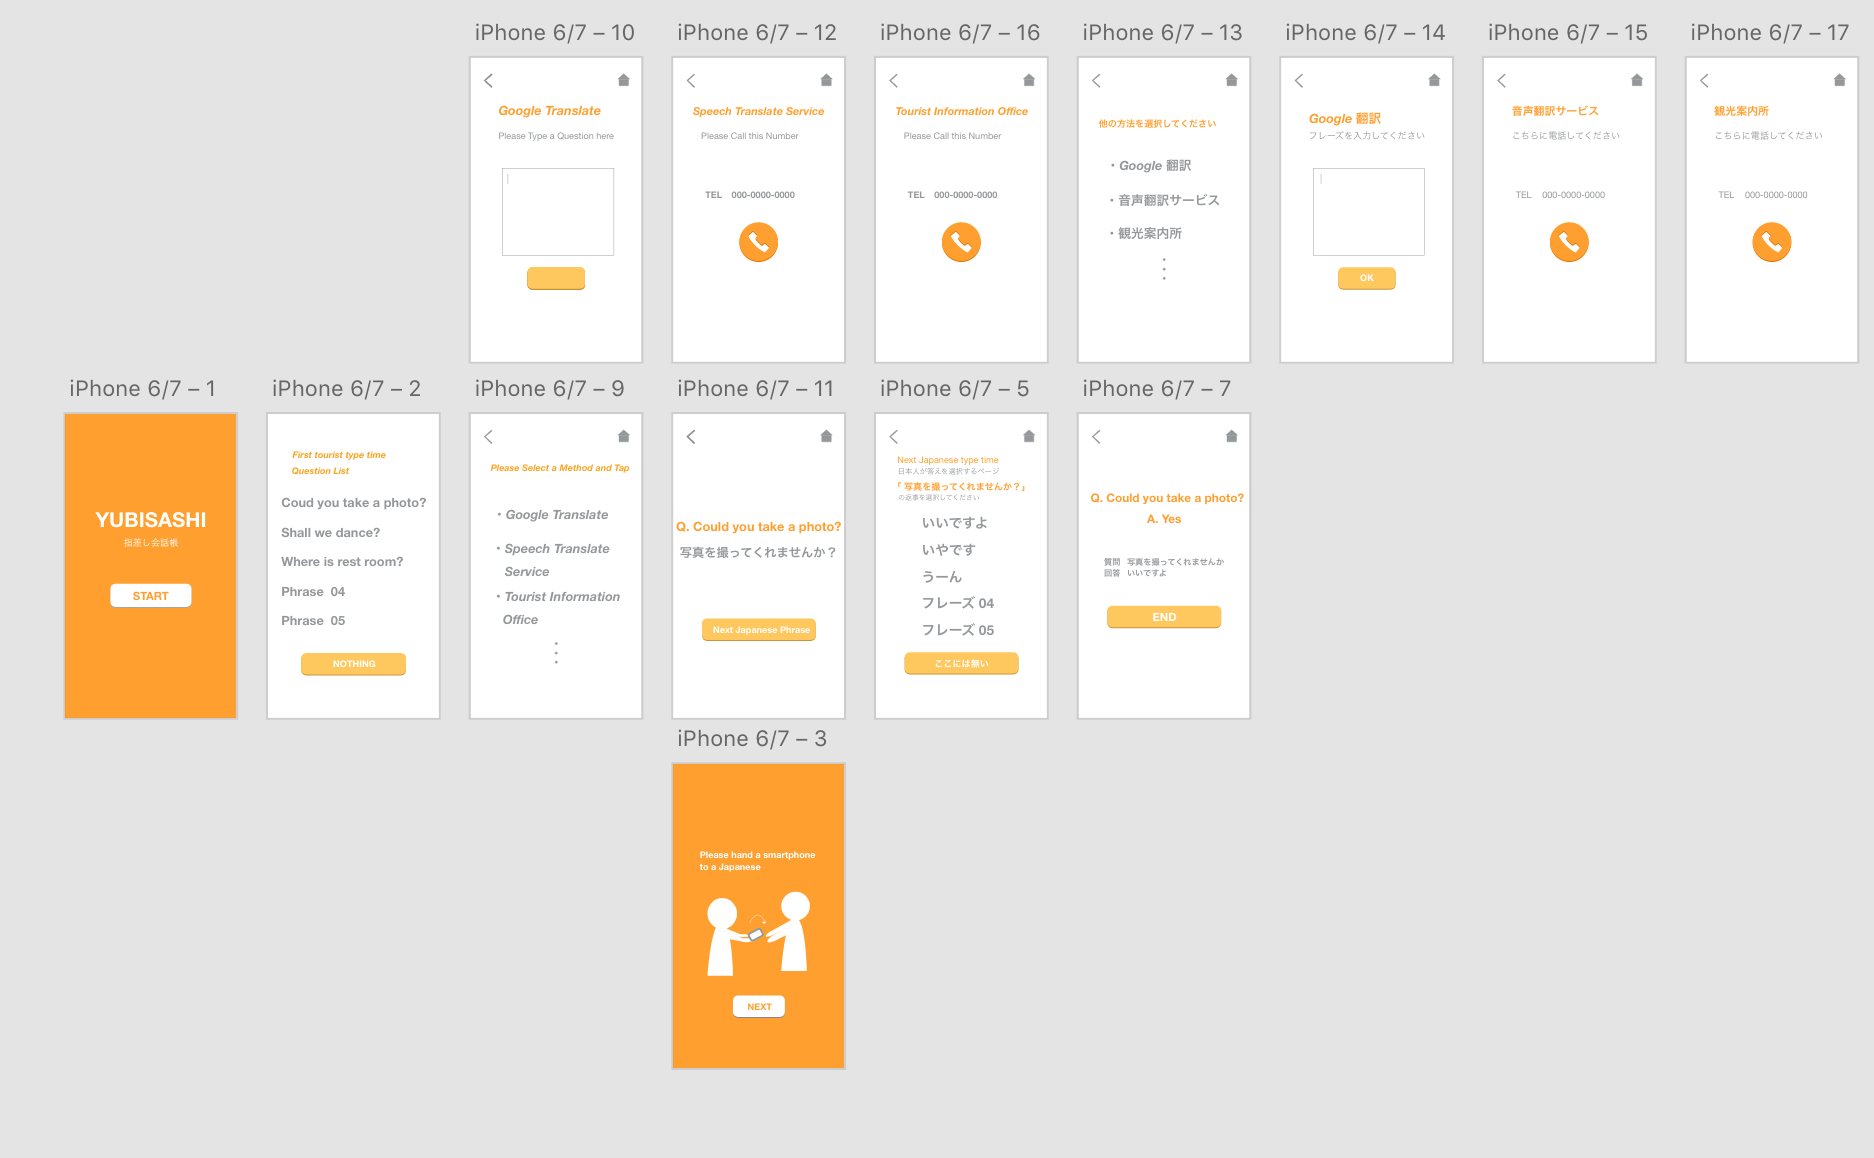
\includegraphics[width=0.75\paperwidth]{img/screen_sample.png}}
 \end{center}
 \caption{プロトタイプ}
 \label{fig:prototype}
\end{figure}
\bunseki{高橋大輔}


\chapter{中間報告会}

\section{発表形式}
 7月14日に行われた中間発表では、各グループの行ってきた活動を詳細に伝え、後期の活動に活かせるレビューを得ることを目的とした。発表としては、全体のポスターを5分程度で発表し、その後に各グループごとに並列で7分程度の発表を行った。その後は時間の許す限り質疑応答の時間とした。私たちのグループでは、今回制作するアプリのモックアップをスマートフォン上に表示し、会話の流れをわかりやすくした。
\bunseki{荒田啓太郎}

\section{レビュー内容}

\subsection{発表方法についての評価と反省}
 中間発表会で行ったアンケートで非常に多かった意見が、言語対応が英語だけでは函館に来る外国人観光客でこのアプリを使えない人が出て来るため、多言語対応すべきというものであった。私たちの構想では多言語対応させるという案は上がっていたが、スクリプトやポスターには反映されていなかったため、このような意見が非常に多く見られた。よって、最終成果発表ではアプリを多言語対応させ、誤解を招くような発表を行わないようにしたい。
\bunseki{荒田啓太郎}

\subsection{発表内容についての評価と反省}\label{sec:yon}
 中間発表会で行ったアンケートから最も多かったものが、本アプリをどうやって外国人観光客に認知してもらうのかというものであった。今回の発表をするにあたって、外国人観光客には事前に本アプリを入れておいてもらうことを前提としていたため、告知方法には十分な検討が行われていなかった。現状では、外国人観光客の多いであろう空港にビーコンでURLを送信するなどしか上がっておらず、後期では認知度をあげる手段についても深く検討していきたい。会話手法についても多くの意見をいただいた。このアプリは見知らぬ人に自身のスマホを渡す必要があり、そのことに対して不快感を覚えたり、手間だと考える人が非常に多いことがアンケートでわかった。他にも、外国人観光客に突然画面を見せられたときの日本人の反応や、個人の事情や用事などで回答を断られた場合の気持ちなど、本アプリでの会話方法には見直しが必要である。
 そして、本アプリでは会話の成立のために事前にフレーズを用意して、外国人観光客が質問をする際、求めていたフレーズがなかったときに機械翻訳を用いるため、初めから機械翻訳を用いれば良いのではないかという意見をいただいた。また、指さし会話帳というものを参考にしているため、それらの手間を超えないようにする必要があるという意見もいただいた。これらについては私たちも考えていたことである。現状、機械翻訳より優れている点として、コンテキストに応じたフレーズを提案されることが挙げられる。本アプリでは利用者の状況によって提案するフレーズを選択し、それらを利用者に提案することを目標にしている。もしもその中に外国人観光客が求めていたフレーズがあれば、そこに日本人側の回答も用意されているので、機械翻訳に外国人観光客の聞きたい質問、そして日本人の回答を入力する手間が省ける。しかしフレーズがない場合の対処方法が普通の翻訳と変わりないのでそこをどうするのか考えていく必要がある。指さし会話帳については、書籍の指さし会話帳に必要な調べるという手間を省くという目的があるので、フレーズの提案方法については吟味していきたい。
 これらの意見をまとめ、最終成果発表までに検討・解決していくものを以下に記述する。
\begin{itemize}
 \item 本アプリを外国人観光客に入れてもらう手段
 \item 本アプリを用いた会話手法・手順
 \item 機械翻訳や、指さし会話帳より優れたものにするためのUI設計やシステム構成
\end{itemize}
\bunseki{荒田啓太郎}


\chapter{グループBのプロセス}

\section{前期の活動}
  Youbeacommは、初め「みんなで作っていく指さし会話帳」をコンセプトにした内容だった。もしその場にあったフレーズがなかった時、ビーコンの周辺にいる人が翻訳をしてあげ、その内容を手動でフレーズ更新をしていくサービスであった。その内容を~\ref{sec:brushup}~のときに発表を行った結果、他のグループから次のような講評を受けた。
\begin{itemize}
\item 翻訳する人のメリットがない
\item すぐに問題を解決できる人がそばにいなかった場合、問題を始めに抱えた人の疑問は解決されない
\item 既存の機械翻訳との違いは何か
\item 情報は増える一方なのか
\item 細かい質問で会話帳が膨大になりそう
\item 問題を感じた人がその問題を送信してくれるとは限らない
\end{itemize}
これらの意見をもとに、もし見合ったフレーズがなかった場合、コンテキストにあった機械翻訳をすることや、観光案内所に繋ぐなどといった対策を考えた。フレーズについても、よく使われるものは、スマートフォン内画面の上部の方に移動して見えやすくするなどの工夫を入れることを改善案にした。改善案を用いて、~\ref{sec:brushup}~のときに発表した結果、協力企業から次のような講評をいただいた。
\begin{itemize}
\item 全てのお客さんの全てのニーズに適応するのは不可能なので、AIを用いてシステムが自ら賢くなる必要がある。如何に学習して提案するかが重要である。
\item この手のものは現場にメリットが大きい。(自動化につながる)GPSでも出来てしまうので、空港の中での詳細な場所で提供すると良いのではないか。
\end{itemize}
ここでいただいた意見を参考にし、中間発表会のポスターに取り入れた。
\bunseki{河田歩美}

\section{後期の活動}
 まず初めに後期の活動の流れとしては、提案した案の見直しをして、簡単なプロトタイプを作り、その後アプリケーション開発を進めていく。開発し後は、アプリケーションを実際に使用してもらい、そのフィードバックから改善を行っていく予定だ。次にプロセスに沿って詳しい説明をしていく。後期の初めに、前期の中間発表で提案したアイデアに、発表を聞いていただいた方々のフィードバックを取り入れ、提案の改善を行っていく。次に、改善した内容をもとにシステムを作っていく。ここで重要視されるのが、~\ref{sec:yon}~にあるように、サーバーが利用者の位置情報や周辺環境を推定したコンテキストと用意されているフレーズとマッチングさせることである。ここでは、既存の利用できるシステムを用いて、本グループが理想とするシステムを開発していく。今回開発をしていくうえで、一番難しいとされているのは適切なフレーズがなかった場合である。この場合、既存の機械翻訳や電話による通訳サービスに繋いだ後、利用者もしくは自動でフレーズの追加を行ってくれるようなシステムにしない限り、フレーズの充実や提案制度の向上を図ることができない。そのため、この点をどう解決できるか後期の活動にかかっている。アプリケーションの開発は、メンバー同士の考えに相違点が生じないよう何度も内容を確認し合いながら開発を行う。アプリケーションの開発後は、函館市の協力のもと実際に函館市内にビーコンを設置し、観光地にいる外国人観光客と市内に住む日本人にアプリケーションを使用してもらう。その際使ってみた感想や改善点を聞き、再びアプリケーションの改善を行う。アプリケーションの改善と実際に使用してもらうことを何度か繰り返し行うことによって本グループの提案するサービスの完成度を上げていく。
\bunseki{河田歩美}


\chapter{前期の振り返りと学び}

\section{振り返り}

\subsection{スケジュール管理}
スケジュール管理は、プロジェクトリーダがプロジェクト開始時に決定した年間スケジュールをもとに管理を行った。前期の活動では、グループリーダが提出物の期限や活動内容、到達目標を管理したことで、年間スケジュールと概ね一致した活動や成果を出すことができた。そのため適切な管理を行えていたといえる。
しかし、グループリーダが作成したスケジュールを早い段階から全体に公開していなかったという問題点があった。
これによって、メンバーの多数が今自分が何をやっているのかについての理解に時間を要してしまった。
後期のプロジェクトでは、プロジェクトリーダとグループリーダ、メンバーとの情報共有の方法を見直し、意見交換会を実施することで認識の齟齬を無くすことが重要であるといえる。
\bunseki{藤原祐汰}

\subsection{情報共有}
私たちは、本プロジェクトが始まった当初、議題に対してプロジェクト全体で発表や共有、意見の交換を行っていた。
しかし、大人数で作業を行う際、アウトプットされる意見が少ないという問題点があった。
そこで、私たちは3人から4人の小グループを作り、そこで討論を行なう手法を用いた。
人数を絞ることで個人が意見を出しやすい環境を作り、議論の効率化を図ったことにより、
より多くの意見をアウトプットさせることが出来た。
よって、私たちが後期のプロジェクト学習を行うに当たって、
小グループでのディスカッションを多く取り入れることが今後も重要になってくると考えられる。
\bunseki{藤原祐汰}

\section{学び}

\subsection{システム設計}
私たちは、前期のプロジェクトを通してより実践的にどのようにしてシステムを設計するのかを学ぶことが出来た。
プロジェクト内でシステム設計についての考え方や、本学の講義であるソフトウェア設計論Ⅰ・Ⅱで学んだ技術を用いて実際に提案したサービスの設計を行った。
実際にグループで考えたサービスのシステムを考え、改善していくことにより、全体を通してより実践的なシステム開発技術を習得できたといえる。
\bunseki{藤原祐汰}

\subsection{情報をアウトプットする技術}
 私たちは、前期のプロジェクトを通して積極的に情報のアウトプットを行ってきた。
ブレーンストーミングやアイデアソンを通して、メンバー個人が保有している情報や発想の洗い出しを行った。
また、外部企業のアドバイザーを招いてのアイデアコンテストや、函館市のものづくり企業紹介の場へ参加し、自らの提案を積極的に外部へアウトプットした。
これらの経験により、プレゼンテーションを行うスキルが上達した。さらにビーコンを知らない人達にビーコンの技術を知ってもらうためには、どのような情報が必要なのか知ることができた。その情報をメンバー間で共有することで全体としてアウトプット技術の向上を図ることが出来た。 
\bunseki{藤原祐汰}

% 以降、付録(付属資料)であることを示す
\begin{appendix}

\chapter{中間報告会で使用したグループBのポスター}
\begin{figure}[htbp]
 \begin{center}
  \makebox[\textwidth]{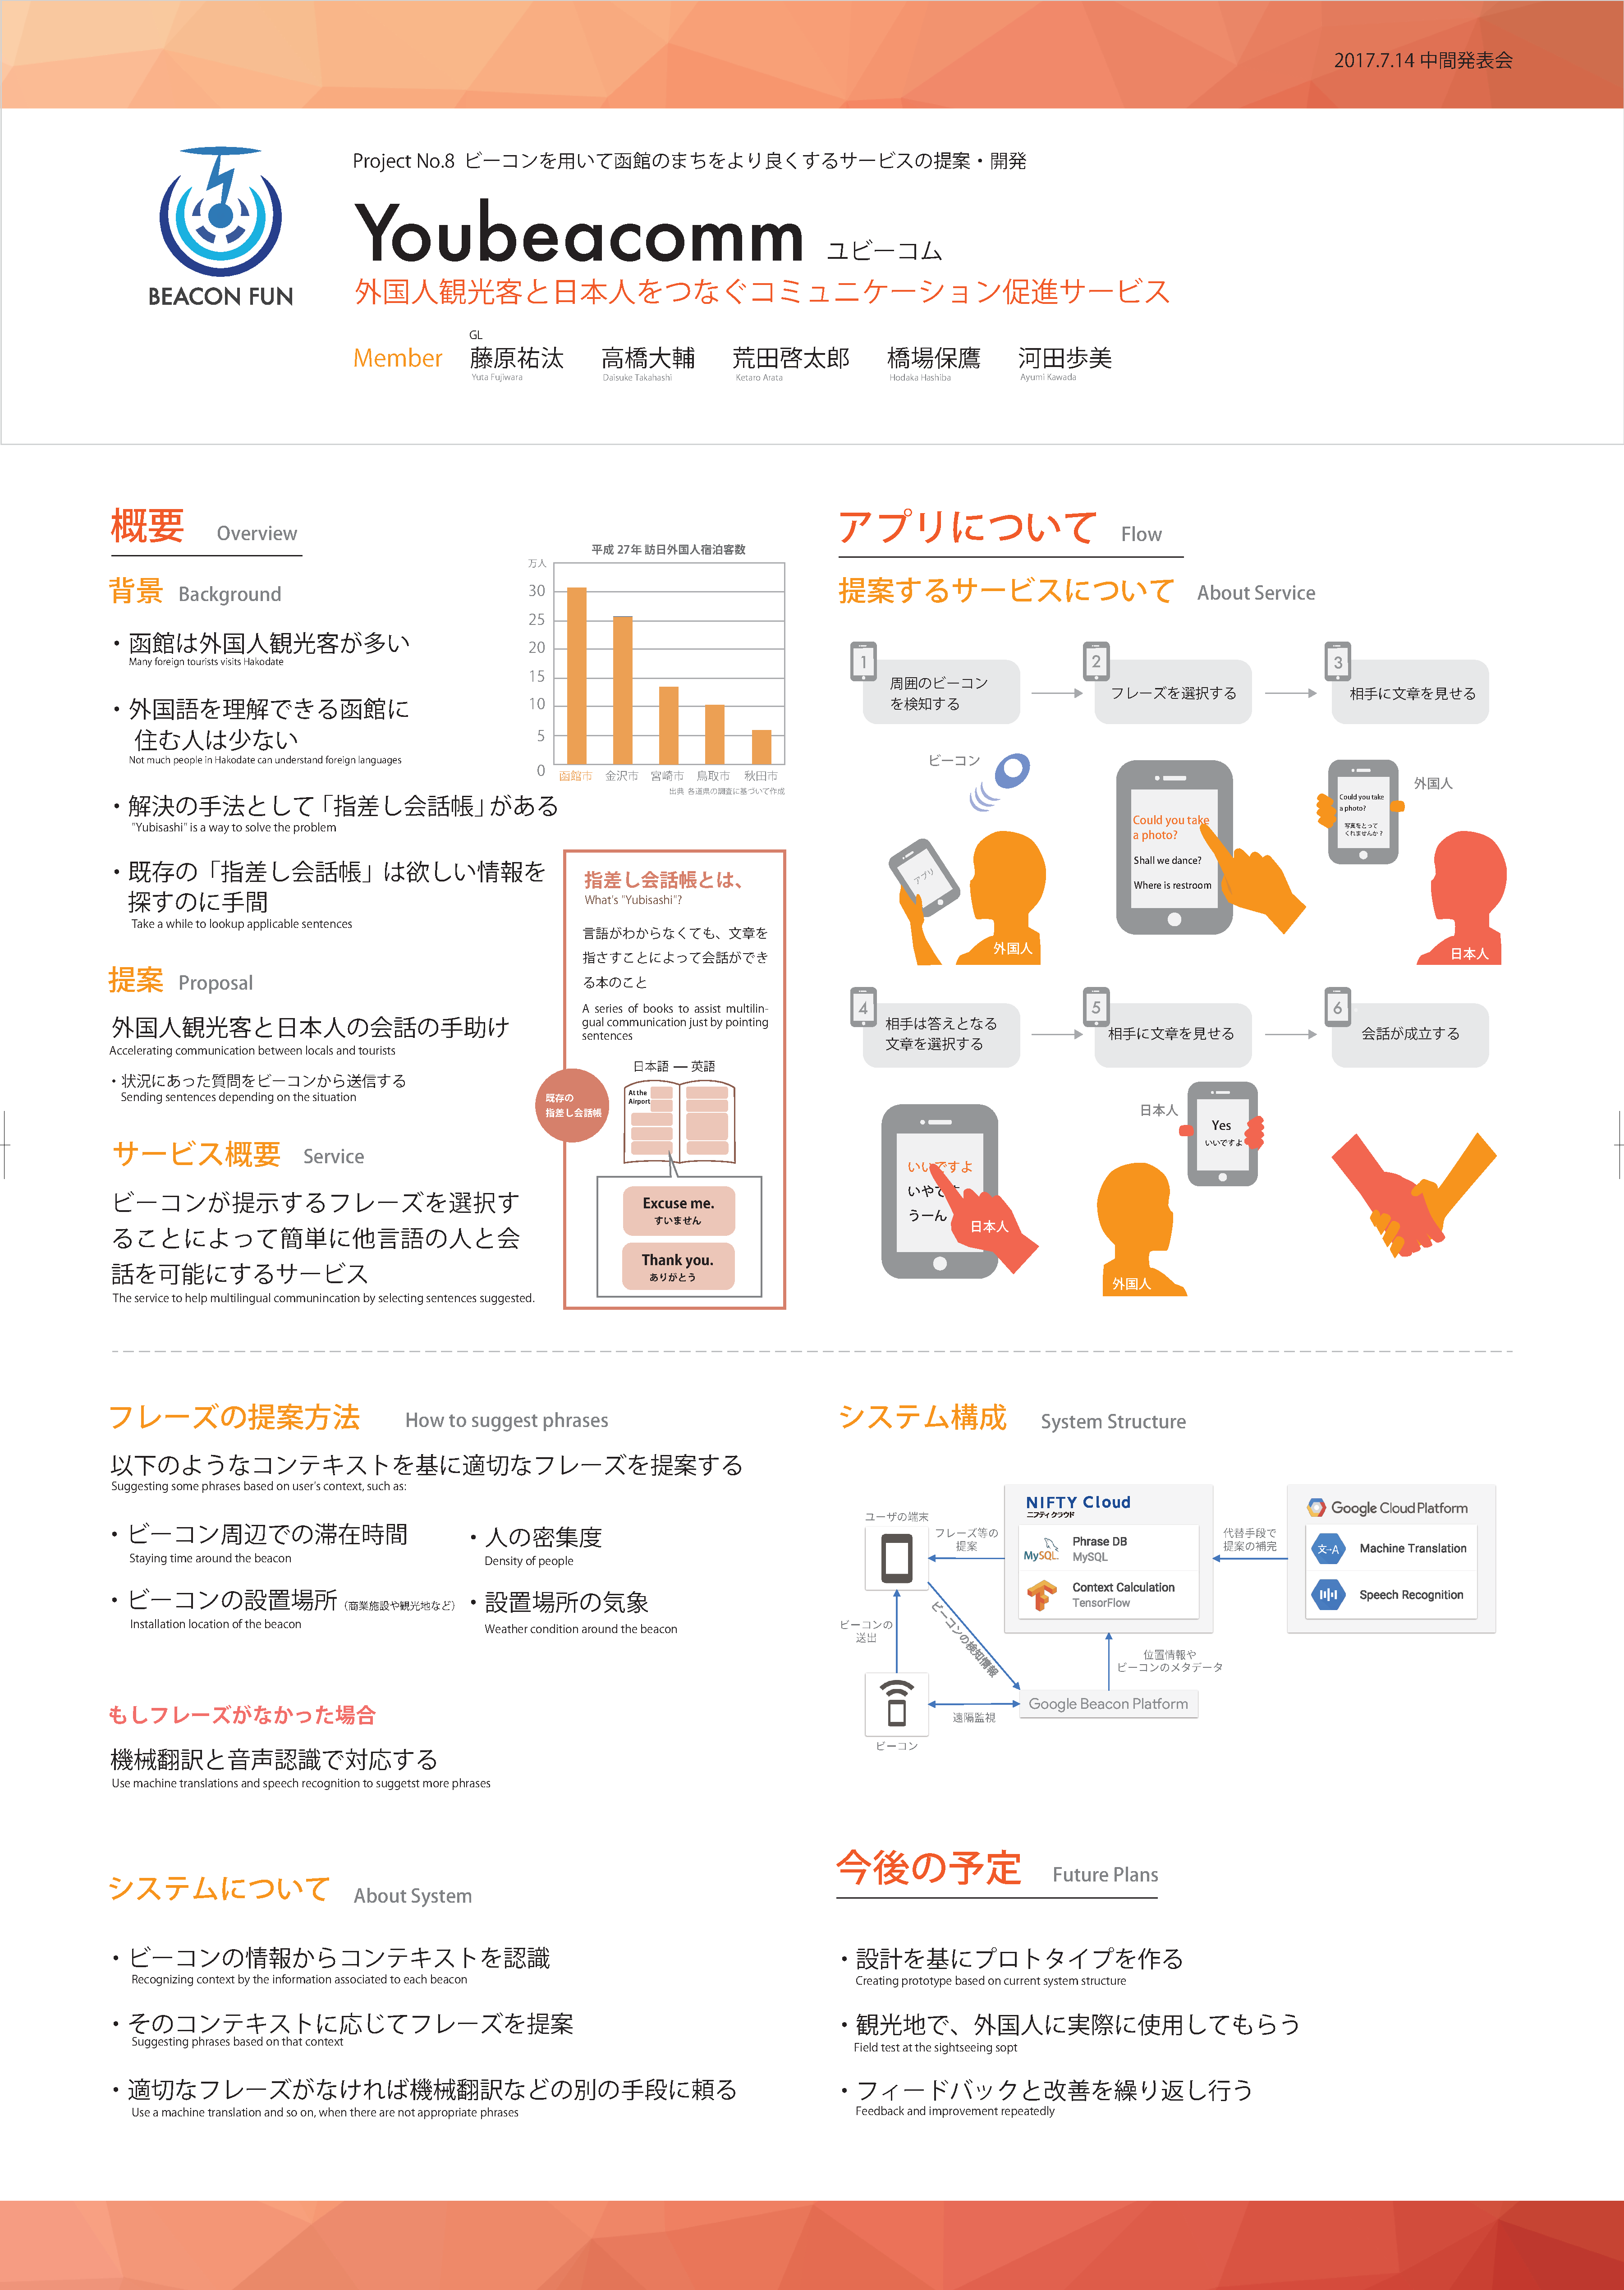
\includegraphics[width=0.714\paperwidth]{img/mid_poster.pdf}}
 \end{center}
\end{figure}

\chapter{中間報告会でもらったコメント一覧}
\begin{itemize}
 \item ビーコンの特徴のような局所性が使うたびに深められる提案がもっと深く掘り下げられると良かった
 \item 会話のきっかけには良いと思った。きっかけを生んだ後のサポートが欲しいと思う(無いと少し困るかも)
 \item 使用するアカウントの言語設定して、日本人も能動的に使えると良いと思いました。不便だと思う機能は、対応言語が英語のみ?中国語や韓国後も対応できればすごい良いと思います
 \item 使用するフレーズがなかった場合に不便だと思った。
 \item 工夫次第で面白くなると思います
 \item 指さし会話帳を知らない日本人もいるのでいきなりそのアプリを起動してスマホを渡されてもアプリの使い方がわからない時に戸惑うと思うので、そのようなことが使い方などを認知してもらう。選択肢が出てこない言葉を伝える方法がとりたい
 \item Could you take a photo?と聞いて、「うーん」って答えたら次はどうなるんでしょうか?ビーコンならではのキラーアプリがあると良いですね。
 \item 何ヶ国語に対応することを考えているか。スマホのやりとりには時間がかかりすぎでは?直接の言語での通訳に変わるものとなるか
 \item コミュニケーションのサポートは大事だと考えた。英語だけでは厳しいのでは?
 \item 言語はなんなのか?英語だけだとわからない人がいるのでは?返答に「いいですよ」とあるけど、okとかsorryくらいは言えるからいらないのでは?どうやって観光客に知ってもらうのか?
 \item 実際にスマホを渡したりすることにためらいを感じる外国人が多いと思うので、そこを払拭して欲しい
 \item どうアプリをダウンロードするか。面白い取り組みだと思うので後期に引き続き頑張ってください
 \item 英和や和英、その他のアプリを使えば例として出てきた函館山などの出来事のように相手に色々携帯を渡すなどの手順を踏む必要がないと思った。このアプリができた時、どうやって宣伝したりするのか
 \item 面白いアプリだと思うが、通信環境がないときに機械翻訳はどう機能するのか。後必ずしも英語が使える外国人がいるとは限らないと思う。ダウンロード方法をどうするか
 \item ビーコンから、ユーザがなんで困っているのかの判断するのが難しそうだなと思いました。うまく判断できれば実用性がありそうだなと思いました
 \item 欲しい選択を本当に受け取れるのか?アプリをどう広めるのか
 \item 会話をするための利用者の使うための意識。でもの画面はディスプレイでやったほうが見やすい
 \item 候補のフレーズを選ぶ手間が会話帳の手間を超えないように頑張って欲しい。絵を入れるのはどうなんですか?
 \item システムとしては面白かったです。返答パターンはもう少し吟味したほうが良いと思います
 \item テキストだけでなくイラストや動画、音を使うと会話がさらに成立しそうと思った
 \item わかりやすかったです
 \item なぜ解決方法として指さし会話帳を選んだのか(他の方法にない具体的な根拠がない)
 \item 質疑に十分な対応ができていた
 \item ポスター、プレゼントもにわかりやすい内容で良かった。実際にサービスが始まったら面白そう
 \item プロトタイプのデモがこの発表でできているのはすごい

\end{itemize}
%付録の終わり
\end{appendix}


%\backmatter

% 参考文献
\printbibliography[title=参考文献]

\end{document}
